\documentclass{article}
\usepackage[utf8]{inputenc}
\usepackage{amsmath}
\usepackage{amssymb}
\usepackage{graphicx}

\newcommand{\comment}[1]{}

\title{Final Project Team 6}
\author{Berenice, Gabriela, Juan, Héctor, Damián}
\date{May 2021}

\begin{document}
    \maketitle
    \tableofcontents
    \newpage



    \begin{abstract}
        The hypothesis of this theorem is that we have a function $F$ that is continuous in a closed interval $[a, b]$, differentiable in the open interval $(a, b)$ and whose values in its extremes $F(a)$ and $F(b)$ match.
        The thesis of the theorem is that, in this case, the derived function vanishes at some point in the interval $(a, b)$
        Notice that since the interval is closed, it makes sense to talk about both $F(a)$ and $F(b)$. We will see that, intuitively, this statement is very simple.
        Rolle's theorem guarantees us that, under these conditions, there must be at least a certain value $x$ of the interval $(a, b)$ for which $F'(x) = 0$. But it only assures us that there has to be that value, not tells us nothing about its how to find it.

        This will be necessary for the problem, because it has a great complexity and will make us develop different mathematical skills to understand how the application of integrals and derivatives works.
    \end{abstract}

    \section{Problem}
    Let $f$ be a three times differentiable function (defined on $\mathbb{R}$
    and real-valued) such that $f$ has at least five distinct real zeros. 
    Prove that $f + 6f' + 12f'' + 8f'''$ has at least two distinct real zeros.
    

    \subsection{Polynomial Function}
    A polynomial is generally represented as $P(x)$. The highest power of the variable of $P(x)$ is known as its degree. Degree of a polynomial function is very important as it tells us about the behaviour of the function $P(x)$ when x becomes very large, and also helps us to know the number of roots that we can have in a function. The domain of a polynomial function is entire real numbers $\mathbb{R} $.

    \comment{
    \section*{Rolle's Thorem}
    Let $f$ be a continuous function on $[a, b]$ and differentiable on $]a, b[$ such that $f(a) = f(b)$. Then there exists $c \in ]a, b[ $ such that $f'(c) = 0$.

    This theorem will be admitted because its proof requires results which are not seen in this course. If $f$ is the constant function, the result is obvious. Otherwise, since $f$ is continuous over $[a, b]$, $f$ is bounded over $[a, b]$
    and reaches its bounds. This means that there exists $m \in  [a, b] $ and $M \in  [a, b] $ such that $\forall x \in  [a, b]$, $f(m) \leqslant  f(x) \leqslant f(M) (f(m) \neq  f(M)$ because $f$ is not a constant function$)$. As $f(a) = f(b)$, then we have the following cases:

    \begin{enumerate}
        \item if $m = a$ or $m = b$, then $M \in  ]a, b[$, hence we have $c = M$;
        \item if $M = a$ or $M = b$, then $m \in  ]a, b[$, hence we have $c = m$;
        \item $m \in  ]a, b[$ and $M \in  ]a, b[$, hence we have $c = m$ or $c = M$.
    \end{enumerate}

    So in all cases $f$ admits a local extremum at a point $c$ of $]a, b[$ and is differentiable on $]a, b[$, hence, according to the proposition 22, $f'(c) = 0$.
    \section*{Hint}
    Use $g : x \rightarrow  e^ {\alpha x} $
    }

    \subsection{Rolle's Theorem}
    Suppose $f(x)$ is a function that satisfies all of the following.
    $f(x)$ is continuous on the closed interval $[a,b]$.
    $f(x)$ is differentiable on the open interval $(a,b)$.
    $$f(a) = f(b)$$
    Then there is a number c such that $a<c<b$ and $f'(c)=0$. Or, in other words $f(x)$ has a critical point in $(a,b)$.

    \begin{figure}[htb]
        \centering
        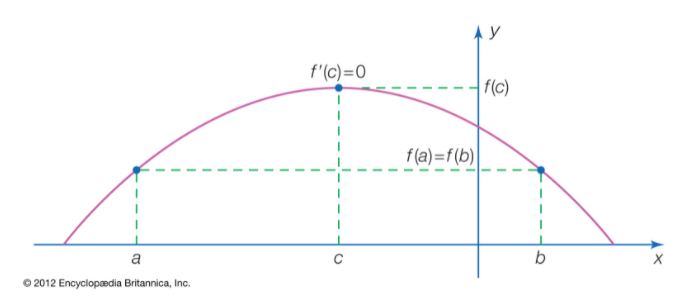
\includegraphics[width=340px]{img/rollestheorem.png}
        \caption{Graphic of Rolle's Theorem}
    \end{figure}

    In other words, if a continuous curve passes through the same y-value (such as the x-axis) twice and has a unique tangent line (derivative) at every point of the interval, then somewhere between the endpoints it has a tangent parallel to the x-axis. The theorem was proved in 1691 by the French mathematician Michel Rolle, though it was stated without a modern formal proof in the 12th century by the Indian mathematician Bhaskara II. Other than being useful in proving the mean-value theorem, Rolle’s theorem is seldom used, since it establishes only the existence of a solution and not its value.

    This theorem helps us to know how many roots (distinct zeros) our function will have once we have derived it three times.

    \subsection{Exponential Function}
    An exponential function is a Mathematical function in form $f(x) = a^x$, where $x$ is a variable and $a$ is a constant which is called the base of the function and it should be greater than $0$. The most commonly used exponential function base is the transcendental number $e$, which is approximately equal to $2.71828$.
    
    An exponential function is defined by the formula $f(x) = a^x$, where the input variable x occurs as an exponent. The exponential curve depends on the exponential function and it depends on the value of the x.

    The exponential function is an important mathematical function which is of the form

    $$f(x) = a^x$$

    Where $a > 0$ and is not equal to $1$.

    $x$ is any real number.

    If the variable is negative, the function is undefined for $-1 < x < 1$.

    \pagebreak
    Here,
    $x$ is a variable
    $a$ is a constant, which is the base of the function.

    An exponential curve grows, or decay depends on the exponential function. Any quantity that grows or decays by a fixed per cent at regular intervals should possess either exponential growth or exponential decay.

    \section{Solution}

\end{document}